\PassOptionsToPackage{unicode=true}{hyperref} % options for packages loaded elsewhere
\PassOptionsToPackage{hyphens}{url}
%
\documentclass[
]{article}
\usepackage{lmodern}
\usepackage{amssymb,amsmath}
\usepackage{ifxetex,ifluatex}
\ifnum 0\ifxetex 1\fi\ifluatex 1\fi=0 % if pdftex
  \usepackage[T1]{fontenc}
  \usepackage[utf8]{inputenc}
  \usepackage{textcomp} % provides euro and other symbols
\else % if luatex or xelatex
  \usepackage{unicode-math}
  \defaultfontfeatures{Scale=MatchLowercase}
  \defaultfontfeatures[\rmfamily]{Ligatures=TeX,Scale=1}
  \setmainfont[]{Verdana}
\fi
% use upquote if available, for straight quotes in verbatim environments
\IfFileExists{upquote.sty}{\usepackage{upquote}}{}
\IfFileExists{microtype.sty}{% use microtype if available
  \usepackage[]{microtype}
  \UseMicrotypeSet[protrusion]{basicmath} % disable protrusion for tt fonts
}{}
\makeatletter
\@ifundefined{KOMAClassName}{% if non-KOMA class
  \IfFileExists{parskip.sty}{%
    \usepackage{parskip}
  }{% else
    \setlength{\parindent}{0pt}
    \setlength{\parskip}{6pt plus 2pt minus 1pt}}
}{% if KOMA class
  \KOMAoptions{parskip=half}}
\makeatother
\usepackage{xcolor}
\IfFileExists{xurl.sty}{\usepackage{xurl}}{} % add URL line breaks if available
\IfFileExists{bookmark.sty}{\usepackage{bookmark}}{\usepackage{hyperref}}
\hypersetup{
  pdftitle={ggplot2},
  pdfauthor={Fabian Koch},
  pdfborder={0 0 0},
  breaklinks=true}
\urlstyle{same}  % don't use monospace font for urls
\usepackage[margin=1in]{geometry}
\usepackage{color}
\usepackage{fancyvrb}
\newcommand{\VerbBar}{|}
\newcommand{\VERB}{\Verb[commandchars=\\\{\}]}
\DefineVerbatimEnvironment{Highlighting}{Verbatim}{commandchars=\\\{\}}
% Add ',fontsize=\small' for more characters per line
\usepackage{framed}
\definecolor{shadecolor}{RGB}{248,248,248}
\newenvironment{Shaded}{\begin{snugshade}}{\end{snugshade}}
\newcommand{\AlertTok}[1]{\textcolor[rgb]{0.94,0.16,0.16}{#1}}
\newcommand{\AnnotationTok}[1]{\textcolor[rgb]{0.56,0.35,0.01}{\textbf{\textit{#1}}}}
\newcommand{\AttributeTok}[1]{\textcolor[rgb]{0.77,0.63,0.00}{#1}}
\newcommand{\BaseNTok}[1]{\textcolor[rgb]{0.00,0.00,0.81}{#1}}
\newcommand{\BuiltInTok}[1]{#1}
\newcommand{\CharTok}[1]{\textcolor[rgb]{0.31,0.60,0.02}{#1}}
\newcommand{\CommentTok}[1]{\textcolor[rgb]{0.56,0.35,0.01}{\textit{#1}}}
\newcommand{\CommentVarTok}[1]{\textcolor[rgb]{0.56,0.35,0.01}{\textbf{\textit{#1}}}}
\newcommand{\ConstantTok}[1]{\textcolor[rgb]{0.00,0.00,0.00}{#1}}
\newcommand{\ControlFlowTok}[1]{\textcolor[rgb]{0.13,0.29,0.53}{\textbf{#1}}}
\newcommand{\DataTypeTok}[1]{\textcolor[rgb]{0.13,0.29,0.53}{#1}}
\newcommand{\DecValTok}[1]{\textcolor[rgb]{0.00,0.00,0.81}{#1}}
\newcommand{\DocumentationTok}[1]{\textcolor[rgb]{0.56,0.35,0.01}{\textbf{\textit{#1}}}}
\newcommand{\ErrorTok}[1]{\textcolor[rgb]{0.64,0.00,0.00}{\textbf{#1}}}
\newcommand{\ExtensionTok}[1]{#1}
\newcommand{\FloatTok}[1]{\textcolor[rgb]{0.00,0.00,0.81}{#1}}
\newcommand{\FunctionTok}[1]{\textcolor[rgb]{0.00,0.00,0.00}{#1}}
\newcommand{\ImportTok}[1]{#1}
\newcommand{\InformationTok}[1]{\textcolor[rgb]{0.56,0.35,0.01}{\textbf{\textit{#1}}}}
\newcommand{\KeywordTok}[1]{\textcolor[rgb]{0.13,0.29,0.53}{\textbf{#1}}}
\newcommand{\NormalTok}[1]{#1}
\newcommand{\OperatorTok}[1]{\textcolor[rgb]{0.81,0.36,0.00}{\textbf{#1}}}
\newcommand{\OtherTok}[1]{\textcolor[rgb]{0.56,0.35,0.01}{#1}}
\newcommand{\PreprocessorTok}[1]{\textcolor[rgb]{0.56,0.35,0.01}{\textit{#1}}}
\newcommand{\RegionMarkerTok}[1]{#1}
\newcommand{\SpecialCharTok}[1]{\textcolor[rgb]{0.00,0.00,0.00}{#1}}
\newcommand{\SpecialStringTok}[1]{\textcolor[rgb]{0.31,0.60,0.02}{#1}}
\newcommand{\StringTok}[1]{\textcolor[rgb]{0.31,0.60,0.02}{#1}}
\newcommand{\VariableTok}[1]{\textcolor[rgb]{0.00,0.00,0.00}{#1}}
\newcommand{\VerbatimStringTok}[1]{\textcolor[rgb]{0.31,0.60,0.02}{#1}}
\newcommand{\WarningTok}[1]{\textcolor[rgb]{0.56,0.35,0.01}{\textbf{\textit{#1}}}}
\usepackage{graphicx,grffile}
\makeatletter
\def\maxwidth{\ifdim\Gin@nat@width>\linewidth\linewidth\else\Gin@nat@width\fi}
\def\maxheight{\ifdim\Gin@nat@height>\textheight\textheight\else\Gin@nat@height\fi}
\makeatother
% Scale images if necessary, so that they will not overflow the page
% margins by default, and it is still possible to overwrite the defaults
% using explicit options in \includegraphics[width, height, ...]{}
\setkeys{Gin}{width=\maxwidth,height=\maxheight,keepaspectratio}
\setlength{\emergencystretch}{3em}  % prevent overfull lines
\providecommand{\tightlist}{%
  \setlength{\itemsep}{0pt}\setlength{\parskip}{0pt}}
\setcounter{secnumdepth}{-2}
% Redefines (sub)paragraphs to behave more like sections
\ifx\paragraph\undefined\else
  \let\oldparagraph\paragraph
  \renewcommand{\paragraph}[1]{\oldparagraph{#1}\mbox{}}
\fi
\ifx\subparagraph\undefined\else
  \let\oldsubparagraph\subparagraph
  \renewcommand{\subparagraph}[1]{\oldsubparagraph{#1}\mbox{}}
\fi

% set default figure placement to htbp
\makeatletter
\def\fps@figure{htbp}
\makeatother

\setlength{\columnsep}{18pt}
\usepackage{multicol}
\newcommand{\hideFromPandoc}[1]{#1}
\hideFromPandoc{ \let\Begin\begin \let\End\end }

\title{ggplot2}
\usepackage{etoolbox}
\makeatletter
\providecommand{\subtitle}[1]{% add subtitle to \maketitle
  \apptocmd{\@title}{\par {\large #1 \par}}{}{}
}
\makeatother
\subtitle{Options, packages and examples for PDF print}
\author{Fabian Koch}
\date{}

\begin{document}
\maketitle

\newpage 
\tableofcontents

\newpage

\hypertarget{data}{%
\section{Data}\label{data}}

\newpage

\hypertarget{informationen}{%
\section{Informationen}\label{informationen}}

\hypertarget{package-infos-repositories-links}{%
\subsection{package Infos, repositories,
links}\label{package-infos-repositories-links}}

\hypertarget{scales}{%
\subsubsection{scales}\label{scales}}

package zur Berechnung von Skalen, bspw. für Achseneinteilungen etc.

\hypertarget{vorlagen}{%
\section{Vorlagen}\label{vorlagen}}

\hypertarget{color-palettes}{%
\subsection{color palettes}\label{color-palettes}}

\begin{Shaded}
\begin{Highlighting}[]
\CommentTok{# Beispiel für manuelle Festlegung diskreter Variablen}
\NormalTok{PAL_Gliederung_Colour <-}\StringTok{ }\KeywordTok{c}\NormalTok{(}\DataTypeTok{SR =} \StringTok{"blue"}\NormalTok{, }\DataTypeTok{UBZTP =} \StringTok{"orange"}\NormalTok{)}
\NormalTok{PAL_Gebiet_fill <-}\StringTok{ }\KeywordTok{c}\NormalTok{(}\StringTok{"yellow3"}\NormalTok{, }\StringTok{"black"}\NormalTok{, }\StringTok{"grey"}\NormalTok{, }\StringTok{"maroon3"}\NormalTok{) }
\NormalTok{PAL_pal9GnPu <-}\StringTok{ }\KeywordTok{c}\NormalTok{(}\StringTok{"#762a83"}\NormalTok{, }\StringTok{"#9970ab"}\NormalTok{, }\StringTok{"#c2a5cf"}\NormalTok{, }\StringTok{"#e7d4e8"}\NormalTok{, }\StringTok{"#f7f7f7"}\NormalTok{, }\StringTok{"#d9f0d3"}\NormalTok{, }\StringTok{"#a6dba0"}\NormalTok{, }\StringTok{"#5aae61"}\NormalTok{, }\StringTok{"#1b7837"}\NormalTok{)}
\NormalTok{PAL_virpal <-}\StringTok{ }\NormalTok{viridisLite}\OperatorTok{::}\KeywordTok{viridis}\NormalTok{(}\DecValTok{6}\NormalTok{)}
\NormalTok{PAL_col6qual <-}\StringTok{ }\KeywordTok{c}\NormalTok{(}\StringTok{"#66c2a5"}\NormalTok{,}\StringTok{"#fc8d62"}\NormalTok{,}\StringTok{"#8da0cb"}\NormalTok{,}\StringTok{"#e78ac3"}\NormalTok{,}\StringTok{"#a6d854"}\NormalTok{,}\StringTok{"#ffd92f"}\NormalTok{)}
\NormalTok{PAL_div_lowcontrast <-}\StringTok{ }\KeywordTok{c}\NormalTok{(}\StringTok{"#fc8d62"}\NormalTok{,}\StringTok{"#e78ac3"}\NormalTok{,}\StringTok{"#66c2a5"}\NormalTok{, }\StringTok{"#8da0cb"}\NormalTok{,}\StringTok{"#a6d854"}\NormalTok{,}\StringTok{"#ffd92f"}\NormalTok{,}\StringTok{"#e5c494"}\NormalTok{)}
\end{Highlighting}
\end{Shaded}

\hypertarget{themes}{%
\subsection{Themes}\label{themes}}

\href{https://ggplot2.tidyverse.org/reference/theme.html}{Refrence
Manual}

Hier werden themes für unterschiedliche Plot Typen und Größen
festgelegt.

Vorschlag für eine Syntax:\\
theme\_package (ggplot, plotly etc.)\_Plottyp (bspw. map oder
barchart)\_Format(print oder HTML)\_Seitenformat (DINA4 oder A5
etc.)\_SpaltenLayout (1, 2 oder 3-spaltig)

Beispiel für ein Theme für ein ggplot2 plot, Typ Karte, für
Printfassungen im A4 Format, 1-spaltig:\\
theme\_ggplot2\_map\_print\_A4\_1c

ggf. später zu vereinfachen, wenn sich heraustellt, dass keine
individuellen Anpassungen zwischen 1- und 2 spaltig erfolgen müssen

/newpage

\hypertarget{snippets}{%
\subsection{Snippets}\label{snippets}}

\hypertarget{beschriftungen}{%
\subsubsection{Beschriftungen}\label{beschriftungen}}

Copy/Paste Vorlage für labs()

\newpage

\hypertarget{plots}{%
\subsubsection{Plots}\label{plots}}

\hypertarget{karte}{%
\paragraph{Karte}\label{karte}}

\begin{Shaded}
\begin{Highlighting}[]
\NormalTok{mapData <-}\StringTok{ }\NormalTok{data_WorldGeom }\OperatorTok\StringTok{ }
\StringTok{  }\KeywordTok{select}\NormalTok{(}
\NormalTok{    name,}
\NormalTok{    continent,}
\NormalTok{    pop_est,}
\NormalTok{    income_grp,}
\NormalTok{    geometry) }\OperatorTok\StringTok{ }
\StringTok{  }\KeywordTok{filter}\NormalTok{(continent }\OperatorTok{==}\StringTok{ "Asia"}\NormalTok{) }\OperatorTok\StringTok{ }
\StringTok{  }\KeywordTok{mutate}\NormalTok{(}
    \CommentTok{# Vereinigung der 5 Kategorien zu 3}
    \DataTypeTok{income_grp =}\NormalTok{ forcats}\OperatorTok{::}\KeywordTok{fct_collapse}\NormalTok{(income_grp,}
      \DataTypeTok{Hoch =} \KeywordTok{c}\NormalTok{(}
        \StringTok{"1. High income: OECD"}\NormalTok{, }
        \StringTok{"2. High income: nonOECD"}\NormalTok{),}
      \DataTypeTok{Mittel =} \KeywordTok{c}\NormalTok{(}
        \StringTok{"3. Upper middle income"}\NormalTok{, }
        \StringTok{"4. Lower middle income"}\NormalTok{),}
      \DataTypeTok{Niedrig =} \KeywordTok{c}\NormalTok{(}
        \StringTok{"5. Low income"}\NormalTok{)))}
  
\NormalTok{mapPlot <-}\StringTok{ }\KeywordTok{ggplot}\NormalTok{(mapData) }\OperatorTok{+}
\StringTok{    }\CommentTok{# da das data.frame eine geometry Spalte besitzt, kommt geom_sf ohne x und y bzw. Rechts- und Hochwerte aus}
\StringTok{    }\CommentTok{# data.frames mit Rechts- und Hochwerten können über sf::st_as_sf in dieses Format konvertiert werden}
\StringTok{    }\CommentTok{# https://www.rdocumentation.org/packages/sf/versions/0.9-7/topics/st_as_sf}
\StringTok{    }\CommentTok{# https://r-spatial.github.io/sf/reference/st_as_sf.html}
\StringTok{    }\KeywordTok{geom_sf}\NormalTok{(}
      \DataTypeTok{data =}\NormalTok{ mapData, }
      \KeywordTok{aes}\NormalTok{(}\DataTypeTok{fill =}\NormalTok{ income_grp)) }\OperatorTok{+}
\StringTok{    }\CommentTok{# Externe Farbpalette, Beispiel viridis}
\StringTok{    }\CommentTok{# https://www.rdocumentation.org/packages/viridis/versions/0.5.1/topics/scale_color_viridis}
\StringTok{    }\NormalTok{viridis}\OperatorTok{::}\KeywordTok{scale_fill_viridis}\NormalTok{(}
      \CommentTok{# Diskrete Variable (Einkommensgruppen)}
      \DataTypeTok{discrete =} \OtherTok{TRUE}\NormalTok{,}
      \CommentTok{# Umkehr der Palette, damit dunkel = Niedrig}
      \DataTypeTok{direction =} \DecValTok{-1}\NormalTok{) }\OperatorTok{+}
\StringTok{    }\CommentTok{# ggrepel ist ein package, das Beschriftungen oder Labels so ausrichtet, dass es zu keinen Überlappungen kommmt}
\StringTok{    }\NormalTok{ggrepel}\OperatorTok{::}\KeywordTok{geom_label_repel}\NormalTok{(}
      \CommentTok{# man kann die ausgewählte Variable in ggplot vorab mit "subset" filtern}
      \DataTypeTok{data =} \KeywordTok{subset}\NormalTok{(mapData, income_grp }\OperatorTok{==}\StringTok{ "Niedrig"}\NormalTok{), }
      \CommentTok{# ohne stat = "sf_coordinates" kann ggrepel keine "geometry" Angaben verarbeiten}
      \DataTypeTok{stat =} \StringTok{"sf_coordinates"}\NormalTok{,}
      \KeywordTok{aes}\NormalTok{(}
        \DataTypeTok{geometry =}\NormalTok{ geometry,}
        \DataTypeTok{label =}\NormalTok{ name)) }\OperatorTok{+}
\StringTok{    }\CommentTok{# siehe theme settings oben}
\StringTok{    }\KeywordTok{theme_ggplot2_map_print_A4_1C}\NormalTok{() }\OperatorTok{+}
\StringTok{    }\CommentTok{# Beschriftungen}
\StringTok{    }\KeywordTok{labs}\NormalTok{(}
      \DataTypeTok{title =} \StringTok{"Titel"}\NormalTok{,}
      \DataTypeTok{subtitle =} \StringTok{"Untertitel"}\NormalTok{,}
      \DataTypeTok{caption =} \StringTok{"Fußnote"}\NormalTok{,}
      \DataTypeTok{tag =} \StringTok{"label"}\NormalTok{,}
      \DataTypeTok{fill =} \StringTok{"Titel Legende"}\NormalTok{) }\OperatorTok{+}
\StringTok{    }\KeywordTok{xlab}\NormalTok{(}\StringTok{"Beschriftung x"}\NormalTok{) }\OperatorTok{+}
\StringTok{    }\KeywordTok{ylab}\NormalTok{(}\StringTok{"Beschriftung y"}\NormalTok{) }
\end{Highlighting}
\end{Shaded}

\hypertarget{scatter-plot-mit-facet-wrap}{%
\paragraph{Scatter Plot mit Facet
Wrap}\label{scatter-plot-mit-facet-wrap}}

\begin{Shaded}
\begin{Highlighting}[]
\NormalTok{ScatterData <-}\StringTok{ }\NormalTok{data_WorldData }\OperatorTok\StringTok{ }
\StringTok{    }\KeywordTok{select}\NormalTok{(}
\NormalTok{    name,}
\NormalTok{    continent,}
\NormalTok{    inequality,}
\NormalTok{    well_being,}
\NormalTok{    gdp_cap_est,}
\NormalTok{    economy) }\OperatorTok\StringTok{ }
\StringTok{  }\KeywordTok{group_by}\NormalTok{(}
\NormalTok{    continent) }\OperatorTok\StringTok{ }
\StringTok{  }\KeywordTok{mutate}\NormalTok{(}\DataTypeTok{avg_gdp =} \KeywordTok{mean}\NormalTok{(gdp_cap_est, }\DataTypeTok{na.rm =} \OtherTok{TRUE}\NormalTok{)) }\OperatorTok\StringTok{ }
\StringTok{  }\KeywordTok{ungroup}\NormalTok{() }\OperatorTok\StringTok{ }
\StringTok{  }\KeywordTok{drop_na}\NormalTok{() }\OperatorTok\StringTok{ }
\StringTok{  }\KeywordTok{mutate}\NormalTok{(}
    \CommentTok{# Vereinigung der Kategorien}
    \DataTypeTok{economy =}\NormalTok{ forcats}\OperatorTok{::}\KeywordTok{fct_collapse}\NormalTok{(economy,}
      \DataTypeTok{entwickelt =} \KeywordTok{c}\NormalTok{(}
        \StringTok{"1. Developed region: G7"}\NormalTok{, }
        \StringTok{"2. Developed region: nonG7"}\NormalTok{),}
      \DataTypeTok{aufstrebend =} \KeywordTok{c}\NormalTok{(}
        \StringTok{"3. Emerging region: BRIC"}\NormalTok{, }
        \StringTok{"4. Emerging region: MIKT"}\NormalTok{, }
        \StringTok{"5. Emerging region: G20"}\NormalTok{),}
      \StringTok{"nicht-entwickelt"}\NormalTok{ =}\StringTok{ }\KeywordTok{c}\NormalTok{(}
        \StringTok{"6. Developing region"}\NormalTok{, }
        \StringTok{"7. Least developed region"}\NormalTok{))) }
  
\NormalTok{ScatterPlot <-}\StringTok{   }
\StringTok{  }\KeywordTok{ggplot}\NormalTok{(ScatterData) }\OperatorTok{+}
\StringTok{  }\KeywordTok{geom_point}\NormalTok{(}
    \KeywordTok{aes}\NormalTok{(}
\NormalTok{      inequality, }
\NormalTok{      well_being,}
    \CommentTok{# Anordung der Kontinente nach absteigender, durchschnittlicher Bevölkerung}
    \DataTypeTok{colour =}\NormalTok{ forcats}\OperatorTok{::}\KeywordTok{fct_reorder}\NormalTok{(continent, }\KeywordTok{desc}\NormalTok{(avg_gdp))),}
    \DataTypeTok{alpha =} \FloatTok{0.8}\NormalTok{) }\OperatorTok{+}\StringTok{ }
\StringTok{  }\KeywordTok{facet_wrap}\NormalTok{(}
    \OperatorTok{~}\StringTok{ }\NormalTok{economy, }
    \DataTypeTok{nrow =} \DecValTok{2}\NormalTok{) }\OperatorTok{+}
\StringTok{  }\KeywordTok{scale_colour_manual}\NormalTok{(}
    \DataTypeTok{values =}\NormalTok{ PAL_div_lowcontrast,}
    \DataTypeTok{guide =} \KeywordTok{guide_legend}\NormalTok{(}
                      \DataTypeTok{title.position =} \StringTok{"top"}\NormalTok{,}
                      \DataTypeTok{title=}\StringTok{"Kontinente"}\NormalTok{,}
                      \DataTypeTok{direction=}\StringTok{"horizontal"}\NormalTok{,}
                      \DataTypeTok{nrow =} \DecValTok{3}\NormalTok{,}
                      \DataTypeTok{ncol =} \DecValTok{2}\NormalTok{)) }\OperatorTok{+}
\StringTok{  }\KeywordTok{geom_smooth}\NormalTok{(}\KeywordTok{aes}\NormalTok{(}\DataTypeTok{x =}\NormalTok{ inequality, }\DataTypeTok{y =}\NormalTok{ well_being), }\DataTypeTok{method =} \StringTok{"lm"}\NormalTok{) }\OperatorTok{+}
\StringTok{  }\KeywordTok{theme_minimal}\NormalTok{() }\OperatorTok{+}
\StringTok{  }\KeywordTok{xlab}\NormalTok{(}\StringTok{"Wohlbefinden"}\NormalTok{) }\OperatorTok{+}
\StringTok{  }\KeywordTok{ylab}\NormalTok{(}\StringTok{"Ungleichheit"}\NormalTok{) }\OperatorTok{+}
\StringTok{  }\KeywordTok{theme}\NormalTok{(}
    \CommentTok{# Legenden Position, Alternativ: "top", "bottom", "right", "left"}
    \DataTypeTok{legend.position =} \KeywordTok{c}\NormalTok{(}\FloatTok{0.72}\NormalTok{, }\FloatTok{0.27}\NormalTok{),}
    \CommentTok{# Legenden Schrift fett}
    \DataTypeTok{legend.title =} \KeywordTok{element_text}\NormalTok{(}\DataTypeTok{face=}\StringTok{"bold"}\NormalTok{),}
    \CommentTok{# Abstand der Achsentitel zum Achsentext}
    \DataTypeTok{axis.title.x =} \KeywordTok{element_text}\NormalTok{(}\DataTypeTok{margin =} \KeywordTok{margin}\NormalTok{(}\DataTypeTok{t =} \DecValTok{15}\NormalTok{, }\DataTypeTok{r =} \DecValTok{0}\NormalTok{, }\DataTypeTok{b =} \DecValTok{0}\NormalTok{, }\DataTypeTok{l =} \DecValTok{0}\NormalTok{)),}
    \DataTypeTok{axis.title.y =} \KeywordTok{element_text}\NormalTok{(}\DataTypeTok{margin =} \KeywordTok{margin}\NormalTok{(}\DataTypeTok{t =} \DecValTok{0}\NormalTok{, }\DataTypeTok{r =} \DecValTok{15}\NormalTok{, }\DataTypeTok{b =} \DecValTok{0}\NormalTok{, }\DataTypeTok{l =} \DecValTok{0}\NormalTok{)))}
\end{Highlighting}
\end{Shaded}

\hypertarget{population-pyramid-varianten}{%
\paragraph{population Pyramid
Varianten}\label{population-pyramid-varianten}}

\hypertarget{data-1}{%
\subparagraph{data}\label{data-1}}

\begin{Shaded}
\begin{Highlighting}[]
\NormalTok{popPyData <-}\StringTok{ }\NormalTok{data_popFM_long }\OperatorTok\StringTok{ }
\StringTok{  }\CommentTok{# filtert Kontinente und Länder Gruppen heraus}
\StringTok{  }\KeywordTok{filter}\NormalTok{(}\OperatorTok{!}\NormalTok{country_code }\OperatorTok{>=}\StringTok{ }\DecValTok{900}\NormalTok{) }\OperatorTok\StringTok{ }
\StringTok{  }\NormalTok{dplyr}\OperatorTok{::}\KeywordTok{group_by}\NormalTok{(}
\NormalTok{    year,}
\NormalTok{    country,}
\NormalTok{    gender) }\OperatorTok\StringTok{ }
\StringTok{  }\NormalTok{dplyr}\OperatorTok{::}\KeywordTok{mutate}\NormalTok{(}
    \DataTypeTok{percPop_country_gender =} \KeywordTok{round}\NormalTok{(population}\OperatorTok{/}\KeywordTok{sum}\NormalTok{(population)}\OperatorTok{*}\DecValTok{100}\NormalTok{,}\DecValTok{1}\NormalTok{)) }\OperatorTok\StringTok{ }
\StringTok{  }\KeywordTok{ungroup}\NormalTok{() }\OperatorTok\StringTok{ }
\StringTok{  }\KeywordTok{mutate}\NormalTok{(}\DataTypeTok{perc_MF =} \KeywordTok{ifelse}\NormalTok{(gender }\OperatorTok{==}\StringTok{ "F"}\NormalTok{, percPop_country_gender}\OperatorTok{*-}\DecValTok{1}\NormalTok{, percPop_country_gender)) }\OperatorTok\StringTok{ }
\StringTok{  }\KeywordTok{filter}\NormalTok{(}
\NormalTok{    year }\OperatorTok{==}\StringTok{ "2015"}
    \OperatorTok{&}\StringTok{ }\NormalTok{country }\OperatorTok{==}\StringTok{ "Germany"}\NormalTok{)}
\end{Highlighting}
\end{Shaded}

\hypertarget{population-pyramid-with-bar-charts}{%
\subparagraph{Population Pyramid with Bar
Charts}\label{population-pyramid-with-bar-charts}}

\begin{Shaded}
\begin{Highlighting}[]
\NormalTok{data <-}\StringTok{ }\NormalTok{popPyData}
\NormalTok{scale_variable <-}\StringTok{ }\KeywordTok{c}\NormalTok{(}\StringTok{"percPop_country_gender"}\NormalTok{)}

\NormalTok{scale_max <-}\StringTok{   }
\StringTok{  }\NormalTok{data }\OperatorTok\StringTok{ }
\StringTok{  }\KeywordTok{select}\NormalTok{(}\KeywordTok{all_of}\NormalTok{(scale_variable)) }\OperatorTok\StringTok{ }
\StringTok{  }\KeywordTok{distinct}\NormalTok{() }\OperatorTok\StringTok{ }
\StringTok{  }\KeywordTok{max}\NormalTok{() }\OperatorTok\StringTok{ }
\StringTok{  }\KeywordTok{round}\NormalTok{(., }\DecValTok{0}\NormalTok{)}

\NormalTok{theme_ggplot2_popPy_print_A4_1C <-}\StringTok{ }\ControlFlowTok{function}\NormalTok{(...) \{}
  \KeywordTok{theme_minimal}\NormalTok{()}
  \KeywordTok{theme}\NormalTok{(}
    \DataTypeTok{text =} \KeywordTok{element_text}\NormalTok{(}
      \CommentTok{# family = default_font_family,}
      \DataTypeTok{color =}\NormalTok{ default_font_color),}
    \CommentTok{# remove all axes}
    \DataTypeTok{axis.line =} \KeywordTok{element_blank}\NormalTok{(),}
    \DataTypeTok{axis.text.x =} \KeywordTok{element_text}\NormalTok{(}
      \DataTypeTok{size =} \DecValTok{7}\NormalTok{, }\DataTypeTok{hjust =} \DecValTok{0}\NormalTok{,}
      \DataTypeTok{color =}\NormalTok{ default_font_color),}
    \DataTypeTok{axis.text.y =} \KeywordTok{element_text}\NormalTok{(}
      \DataTypeTok{margin =} \KeywordTok{unit}\NormalTok{(}\KeywordTok{c}\NormalTok{(}\DataTypeTok{t =} \DecValTok{0}\NormalTok{, }\DataTypeTok{r =} \FloatTok{-0.7}\NormalTok{, }\DataTypeTok{b =} \DecValTok{0}\NormalTok{, }\DataTypeTok{l =} \DecValTok{0}\NormalTok{), }\StringTok{"cm"}\NormalTok{)),}
    \DataTypeTok{axis.ticks =} \KeywordTok{element_blank}\NormalTok{(),}
    \DataTypeTok{axis.title.y=}\KeywordTok{element_blank}\NormalTok{(),}
    \CommentTok{# panel.grid.major = element_blank(),}
    \CommentTok{# panel.grid.minor = element_blank(),}
    \CommentTok{# background colors}
    \DataTypeTok{plot.background =} \KeywordTok{element_rect}\NormalTok{(}\DataTypeTok{fill =}\NormalTok{ default_background_color,}
                                   \DataTypeTok{color =} \OtherTok{NA}\NormalTok{),}
    \DataTypeTok{panel.background =} \KeywordTok{element_rect}\NormalTok{(}\DataTypeTok{fill =}\NormalTok{ default_background_color,}
                                    \DataTypeTok{color =} \OtherTok{NA}\NormalTok{),}
    \DataTypeTok{legend.background =} \KeywordTok{element_rect}\NormalTok{(}\DataTypeTok{fill =}\NormalTok{ default_background_color,}
                                     \DataTypeTok{color =} \OtherTok{NA}\NormalTok{),}
    \CommentTok{# borders and margins}
    \DataTypeTok{panel.border =} \KeywordTok{element_blank}\NormalTok{(),}
    \DataTypeTok{panel.spacing =} \KeywordTok{unit}\NormalTok{(}\KeywordTok{c}\NormalTok{(}\DecValTok{0}\NormalTok{, }\DecValTok{0}\NormalTok{, }\DecValTok{0}\NormalTok{, }\DecValTok{0}\NormalTok{), }\StringTok{"cm"}\NormalTok{),}
    \CommentTok{# titles}
    \DataTypeTok{legend.title =} \KeywordTok{element_text}\NormalTok{(}\DataTypeTok{size =} \DecValTok{7}\NormalTok{),}
    \DataTypeTok{legend.text =} \KeywordTok{element_text}\NormalTok{(}\DataTypeTok{size =} \DecValTok{7}\NormalTok{, }\DataTypeTok{hjust =} \DecValTok{0}\NormalTok{,}
                               \DataTypeTok{color =}\NormalTok{ default_font_color),}
    \DataTypeTok{plot.title =} \KeywordTok{element_text}\NormalTok{(}\DataTypeTok{size =} \DecValTok{20}\NormalTok{, }
                              \DataTypeTok{color =}\NormalTok{ default_font_color,}
                              \DataTypeTok{face =} \StringTok{"bold"}\NormalTok{),}
    \DataTypeTok{plot.subtitle =} \KeywordTok{element_text}\NormalTok{(}\DataTypeTok{size =} \DecValTok{15}\NormalTok{, }
                                 \DataTypeTok{color =}\NormalTok{ default_font_color,}
                                 \DataTypeTok{margin =} \KeywordTok{margin}\NormalTok{(}\DataTypeTok{b =} \FloatTok{-0.1}\NormalTok{,}
                                                 \DataTypeTok{t =} \FloatTok{-0.1}\NormalTok{,}
                                                 \DataTypeTok{l =} \DecValTok{2}\NormalTok{,}
                                                 \DataTypeTok{unit =} \StringTok{"cm"}\NormalTok{),}
                                 \DataTypeTok{debug =}\NormalTok{ F),}
    \CommentTok{# captions}
    \DataTypeTok{plot.caption =} \KeywordTok{element_text}\NormalTok{(}\DataTypeTok{size =} \DecValTok{10}\NormalTok{,}
                                \DataTypeTok{hjust =} \DecValTok{0}\NormalTok{,}
                                \DataTypeTok{margin =} \KeywordTok{margin}\NormalTok{(}\DataTypeTok{t =} \FloatTok{0.2}\NormalTok{,}
                                                \DataTypeTok{b =} \DecValTok{0}\NormalTok{,}
                                                \DataTypeTok{unit =} \StringTok{"cm"}\NormalTok{),}
                                \DataTypeTok{color =} \StringTok{"#939184"}\NormalTok{),}
\NormalTok{    ...}
\NormalTok{  ) }
    
\NormalTok{\}}

\NormalTok{Male <-}\StringTok{ }\KeywordTok{ggplot}\NormalTok{(}
  \DataTypeTok{data =}\NormalTok{ popPyData[popPyData}\OperatorTok{$}\NormalTok{gender}\OperatorTok{==}\StringTok{"M"}\NormalTok{,], }
  \KeywordTok{aes}\NormalTok{(}
    \DataTypeTok{x =}\NormalTok{ percPop_country_gender,}
    \DataTypeTok{y =}\NormalTok{ age)) }\OperatorTok{+}
\StringTok{  }\KeywordTok{geom_col}\NormalTok{(}\DataTypeTok{fill =} \StringTok{"cornflowerblue"}\NormalTok{) }\OperatorTok{+}
\StringTok{  }\KeywordTok{theme_ggplot2_popPy_print_A4_1C}\NormalTok{() }\OperatorTok{+}
\StringTok{  }\KeywordTok{scale_x_continuous}\NormalTok{(}
    \DataTypeTok{name =} \StringTok{""}\NormalTok{, }
    \DataTypeTok{limits =} \KeywordTok{c}\NormalTok{(}\DecValTok{0}\NormalTok{, scale_max), }
    \DataTypeTok{breaks=}\NormalTok{ scales}\OperatorTok{::}\KeywordTok{breaks_pretty}\NormalTok{(}\DecValTok{5}\NormalTok{), }
    \DataTypeTok{expand =} \KeywordTok{c}\NormalTok{(}\DecValTok{0}\NormalTok{, }\DecValTok{1}\NormalTok{)) }\OperatorTok{+}\StringTok{   }
\StringTok{  }\KeywordTok{theme}\NormalTok{(}
    \CommentTok{# durch die umgekehrte Ausrichtung der weiblichen/männlichen Plots}
    \CommentTok{# müssen die margins separat gesetzt werden}
    \DataTypeTok{plot.margin =} \KeywordTok{unit}\NormalTok{(}\KeywordTok{c}\NormalTok{(}\DataTypeTok{t =} \DecValTok{0}\NormalTok{, }\DataTypeTok{r =} \FloatTok{-0.5}\NormalTok{, }\DataTypeTok{b =} \DecValTok{0}\NormalTok{, }\DataTypeTok{l =} \FloatTok{-0.5}\NormalTok{), }\StringTok{"cm"}\NormalTok{)) }\OperatorTok{+}
\StringTok{  }\KeywordTok{ylab}\NormalTok{(}\StringTok{"Anteil"}\NormalTok{) }
   



\NormalTok{Female <-}\StringTok{ }\KeywordTok{ggplot}\NormalTok{(}
  \DataTypeTok{data =}\NormalTok{ popPyData[popPyData}\OperatorTok{$}\NormalTok{gender}\OperatorTok{==}\StringTok{"F"}\NormalTok{,], }
  \KeywordTok{aes}\NormalTok{(}
    \DataTypeTok{x =}\NormalTok{ percPop_country_gender,}
    \DataTypeTok{y =}\NormalTok{ age)) }\OperatorTok{+}
\StringTok{  }\KeywordTok{geom_col}\NormalTok{(}\DataTypeTok{fill =} \StringTok{"darkseagreen2"}\NormalTok{) }\OperatorTok{+}
\StringTok{  }\KeywordTok{theme_ggplot2_popPy_print_A4_1C}\NormalTok{() }\OperatorTok{+}
\StringTok{  }\KeywordTok{scale_x_reverse}\NormalTok{(}
    \DataTypeTok{name =} \StringTok{""}\NormalTok{, }
    \CommentTok{# da Achse für weibliche Personen umgekehrt wird (_reverse)}
    \CommentTok{# muss auch der min und max Wert umgekehrt angegben werden}
    \DataTypeTok{limits =} \KeywordTok{c}\NormalTok{(scale_max, }\DecValTok{0}\NormalTok{), }
    \DataTypeTok{breaks=}\NormalTok{ scales}\OperatorTok{::}\KeywordTok{breaks_pretty}\NormalTok{(}\DecValTok{5}\NormalTok{), }
    \DataTypeTok{expand =} \KeywordTok{c}\NormalTok{(}\DecValTok{0}\NormalTok{, }\DecValTok{1}\NormalTok{)) }\OperatorTok{+}
\StringTok{  }\KeywordTok{theme}\NormalTok{(}
    \CommentTok{# durch die umgekehrte Ausrichtung der weiblichen/männlichen Plots}
    \CommentTok{# müssen die margins separat gesetzt werden}
    \DataTypeTok{plot.margin =} \KeywordTok{unit}\NormalTok{(}\KeywordTok{c}\NormalTok{(}\DataTypeTok{t =} \DecValTok{0}\NormalTok{, }\DataTypeTok{r =} \DecValTok{0}\NormalTok{, }\DataTypeTok{b =} \DecValTok{0}\NormalTok{, }\DataTypeTok{l =} \FloatTok{-0.5}\NormalTok{), }\StringTok{"cm"}\NormalTok{),}
        \DataTypeTok{axis.text.y =} \KeywordTok{element_blank}\NormalTok{()) }\OperatorTok{+}
\StringTok{  }\KeywordTok{ylab}\NormalTok{(}\StringTok{"Angaben in %"}\NormalTok{) }



\NormalTok{gridExtra}\OperatorTok{::}\KeywordTok{grid.arrange}\NormalTok{(}
\NormalTok{  Female,}
\NormalTok{  Male,}
  \DataTypeTok{widths=}\KeywordTok{c}\NormalTok{(}\FloatTok{0.5}\NormalTok{,}\FloatTok{0.5}\NormalTok{),}
  \DataTypeTok{ncol=}\DecValTok{2}\NormalTok{,}
  \CommentTok{# https://www.rdocumentation.org/packages/grid/versions/3.6.2/topics/grid.text}
  \DataTypeTok{top =}\NormalTok{ grid}\OperatorTok{::}\KeywordTok{textGrob}\NormalTok{(}
    \StringTok{"Alterspyramide"}\NormalTok{,}
    \DataTypeTok{hjust =} \DecValTok{3}\NormalTok{,}
    \DataTypeTok{gp=}\NormalTok{grid}\OperatorTok{::}\KeywordTok{gpar}\NormalTok{(}
      \DataTypeTok{fontsize=}\DecValTok{10}\NormalTok{,}
      \DataTypeTok{font=}\DecValTok{2}\NormalTok{)))}
\end{Highlighting}
\end{Shaded}

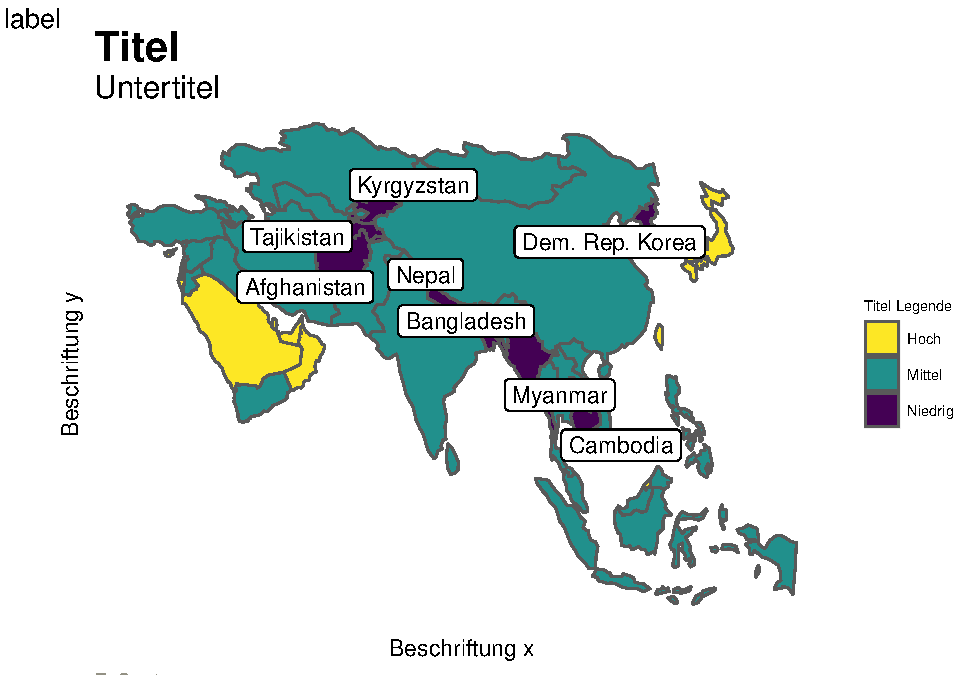
\includegraphics{ggplot2_files/figure-latex/unnamed-chunk-7-1.pdf}

\hypertarget{bar-charts}{%
\paragraph{Bar Charts}\label{bar-charts}}

\begin{Shaded}
\begin{Highlighting}[]
\NormalTok{countryList <-}\StringTok{ }\KeywordTok{c}\NormalTok{(}\StringTok{"Germany"}\NormalTok{,}\StringTok{"Romania"}\NormalTok{,}\StringTok{"Bulgaria"}\NormalTok{,}\StringTok{"Syrian Arab Republic"}\NormalTok{)}

\NormalTok{BarData <-}\StringTok{ }\NormalTok{data_popFM_long }\OperatorTok\StringTok{ }
\StringTok{  }\CommentTok{# filtert Kontinente und Länder Gruppen heraus}
\StringTok{  }\KeywordTok{filter}\NormalTok{(}\OperatorTok{!}\NormalTok{country_code }\OperatorTok{>=}\StringTok{ }\DecValTok{900}\NormalTok{) }\OperatorTok\StringTok{ }
\StringTok{  }\NormalTok{dplyr}\OperatorTok{::}\KeywordTok{group_by}\NormalTok{(}
\NormalTok{    year,}
\NormalTok{    country,}
\NormalTok{    gender) }\OperatorTok\StringTok{ }
\StringTok{  }\NormalTok{dplyr}\OperatorTok{::}\KeywordTok{mutate}\NormalTok{(}
    \DataTypeTok{percPop_country_gender =} \KeywordTok{round}\NormalTok{(population}\OperatorTok{/}\KeywordTok{sum}\NormalTok{(population)}\OperatorTok{*}\DecValTok{100}\NormalTok{,}\DecValTok{1}\NormalTok{)) }\OperatorTok\StringTok{ }
\StringTok{  }\KeywordTok{filter}\NormalTok{(year }\OperatorTok{==}\StringTok{ "2015"}\NormalTok{) }\OperatorTok\StringTok{ }
\StringTok{  }\KeywordTok{filter}\NormalTok{(country }\OperatorTok\StringTok{ }\NormalTok{countryList)}

\NormalTok{plotBarGrouped <-}\StringTok{ }\NormalTok{BarData }\OperatorTok\StringTok{ }
\StringTok{    }\KeywordTok{ggplot}\NormalTok{( }
      \KeywordTok{aes}\NormalTok{(}
        \DataTypeTok{x=}\NormalTok{age, }
        \DataTypeTok{y=}\NormalTok{percPop_country_gender, }
        \DataTypeTok{group=}\NormalTok{gender, }
        \DataTypeTok{fill=}\NormalTok{gender)) }\OperatorTok{+}
\StringTok{    }\KeywordTok{geom_bar}\NormalTok{(}
      \DataTypeTok{position =} \StringTok{"dodge"}\NormalTok{, }\DataTypeTok{width=}\FloatTok{0.7}\NormalTok{,}
      \DataTypeTok{stat =} \StringTok{"identity"}\NormalTok{) }\OperatorTok{+}
\StringTok{    }\KeywordTok{scale_fill_manual}\NormalTok{(}\DataTypeTok{labels =} \KeywordTok{c}\NormalTok{(}\StringTok{"männlich"}\NormalTok{, }\StringTok{"weiblich"}\NormalTok{), }\DataTypeTok{values =} \KeywordTok{c}\NormalTok{(}\StringTok{"cornflowerblue"}\NormalTok{, }\StringTok{"darkseagreen2"}\NormalTok{)) }\OperatorTok{+}
\StringTok{    }\KeywordTok{scale_x_discrete}\NormalTok{(}\DataTypeTok{guide =} \KeywordTok{guide_axis}\NormalTok{(}\DataTypeTok{angle =} \DecValTok{90}\NormalTok{)) }\OperatorTok{+}
\StringTok{    }\KeywordTok{labs}\NormalTok{(}
      \DataTypeTok{title =} \StringTok{"Anteile der Bevölkerung nach Geschlecht und Altersgruppe"}\NormalTok{,}
      \DataTypeTok{subtitle =} \StringTok{"in West-europäischen Ländern, 2015"}\NormalTok{,}
      \DataTypeTok{caption =} \StringTok{"Datenset wpp2015, Age- and sex-specific populationestimates and projections "}\NormalTok{,}
      \DataTypeTok{tag =} \StringTok{"Abb. 01"}\NormalTok{,}
      \DataTypeTok{fill =} \StringTok{"Geschlecht"}\NormalTok{) }\OperatorTok{+}
\StringTok{    }\KeywordTok{xlab}\NormalTok{(}\StringTok{"Altersgruppen"}\NormalTok{) }\OperatorTok{+}
\StringTok{    }\KeywordTok{ylab}\NormalTok{(}\StringTok{"Anteil an geschlechtsspezifischer Hauptwohnbevölkerung"}\NormalTok{) }\OperatorTok{+}
\StringTok{  }\KeywordTok{facet_wrap}\NormalTok{(}\OperatorTok{~}\StringTok{ }\NormalTok{country) }\OperatorTok{+}
\StringTok{  }\KeywordTok{theme_minimal}\NormalTok{()}



\NormalTok{plotBarFill <-}\StringTok{ }\NormalTok{BarData }\OperatorTok\StringTok{ }
\StringTok{    }\KeywordTok{ggplot}\NormalTok{() }\OperatorTok{+}
\StringTok{    }\KeywordTok{geom_bar}\NormalTok{(}
      \CommentTok{# filter des Datensatzes auf weibliche Personen}
      \CommentTok{# Alternative: BarData[BarData$gender=="F",]}
      \DataTypeTok{data =} \KeywordTok{subset}\NormalTok{(BarData, gender }\OperatorTok{==}\StringTok{ "F"}\NormalTok{), }
      \KeywordTok{aes}\NormalTok{(}
        \DataTypeTok{x=}\NormalTok{age, }
        \DataTypeTok{y=}\NormalTok{percPop_country_gender),}
      \DataTypeTok{fill =} \OtherTok{NA}\NormalTok{,}
      \DataTypeTok{color =} \StringTok{"Black"}\NormalTok{,}
      \CommentTok{# position = "identity",}
      \DataTypeTok{stat=}\StringTok{"identity"}\NormalTok{) }\OperatorTok{+}
\StringTok{    }\KeywordTok{geom_bar}\NormalTok{(}
      \DataTypeTok{data =} \KeywordTok{subset}\NormalTok{(BarData, gender }\OperatorTok{==}\StringTok{ "M"}\NormalTok{), }
      \KeywordTok{aes}\NormalTok{(}
        \DataTypeTok{x=}\NormalTok{age, }
        \DataTypeTok{y=}\NormalTok{percPop_country_gender),}
      \DataTypeTok{alpha =} \FloatTok{0.3}\NormalTok{,}
      \CommentTok{# position = "identity",}
      \DataTypeTok{stat=}\StringTok{"identity"}\NormalTok{) }\OperatorTok{+}
\StringTok{    }\KeywordTok{scale_x_discrete}\NormalTok{(}\DataTypeTok{guide =} \KeywordTok{guide_axis}\NormalTok{(}\DataTypeTok{angle =} \DecValTok{90}\NormalTok{)) }\OperatorTok{+}
\StringTok{    }\CommentTok{# scale_colour_manual(labels = c("männlich", "weiblich"), values=gender, aesthetics = c("colour", "fill")) +}
\StringTok{    }\KeywordTok{scale_colour_manual}\NormalTok{(}\DataTypeTok{labels =} \KeywordTok{c}\NormalTok{(}\StringTok{"männlich"}\NormalTok{, }\StringTok{"weiblich"}\NormalTok{), }\DataTypeTok{values=}\KeywordTok{c}\NormalTok{(}\StringTok{"lightblue4"}\NormalTok{, }\StringTok{"red"}\NormalTok{)) }\OperatorTok{+}
\StringTok{    }\KeywordTok{labs}\NormalTok{(}
      \DataTypeTok{title =} \StringTok{"Anteile der Bevölkerung nach Geschlecht und Altersgruppe"}\NormalTok{,}
      \DataTypeTok{subtitle =} \StringTok{"in West-europäischen Ländern, 2015"}\NormalTok{,}
      \DataTypeTok{caption =} \StringTok{"Datenset wpp2015, Age- and sex-specific populationestimates and projections "}\NormalTok{,}
      \DataTypeTok{tag =} \StringTok{"Abb. 01"}\NormalTok{,}
      \DataTypeTok{fill =} \StringTok{"Geschlecht"}\NormalTok{) }\OperatorTok{+}
\StringTok{    }\KeywordTok{xlab}\NormalTok{(}\StringTok{"Altersgruppen"}\NormalTok{) }\OperatorTok{+}
\StringTok{    }\KeywordTok{ylab}\NormalTok{(}\StringTok{"Anteil an geschlechtsspezifischer Hauptwohnbevölkerung"}\NormalTok{) }\OperatorTok{+}
\StringTok{  }\KeywordTok{facet_wrap}\NormalTok{(}\OperatorTok{~}\StringTok{ }\NormalTok{country, }\DataTypeTok{nrow =} \DecValTok{2}\NormalTok{, }\DataTypeTok{ncol =} \DecValTok{2}\NormalTok{) }\OperatorTok{+}
\StringTok{  }\KeywordTok{theme_minimal}\NormalTok{()}


\NormalTok{plotBarOverlay <-}\StringTok{ }\NormalTok{BarData }\OperatorTok\StringTok{ }
\StringTok{    }\KeywordTok{ggplot}\NormalTok{(      }
      \KeywordTok{aes}\NormalTok{(}
        \DataTypeTok{x=}\NormalTok{age, }
        \DataTypeTok{y=}\NormalTok{percPop_country_gender,}
        \DataTypeTok{fill =}\NormalTok{ gender}
        \CommentTok{# color = gender,}
        \CommentTok{# alpha = gender}
\NormalTok{        )) }\OperatorTok{+}
\StringTok{    }\KeywordTok{geom_bar}\NormalTok{(}
      \DataTypeTok{alpha =} \FloatTok{0.6}\NormalTok{,}
      \DataTypeTok{position =} \StringTok{"identity"}\NormalTok{,}
      \DataTypeTok{stat=}\StringTok{"identity"}\NormalTok{) }\OperatorTok{+}
\StringTok{  }\CommentTok{# scale_colour_manual(values=c("lightblue4", "red")) +}
\StringTok{  }\KeywordTok{scale_fill_manual}\NormalTok{(}
    \DataTypeTok{labels =} \KeywordTok{c}\NormalTok{(}\StringTok{"männlich"}\NormalTok{, }\StringTok{"weiblich"}\NormalTok{),}
    \DataTypeTok{values=}\KeywordTok{c}\NormalTok{(}\StringTok{"lightblue"}\NormalTok{, }\StringTok{"pink"}\NormalTok{)) }\OperatorTok{+}
\StringTok{  }\KeywordTok{scale_x_discrete}\NormalTok{(}\DataTypeTok{guide =} \KeywordTok{guide_axis}\NormalTok{(}\DataTypeTok{angle =} \DecValTok{90}\NormalTok{)) }\OperatorTok{+}
\StringTok{  }\CommentTok{# scale_alpha_manual(values=c(.3, .8)) +}
\StringTok{    }\KeywordTok{labs}\NormalTok{(}
      \DataTypeTok{title =} \StringTok{"Anteile der Bevölkerung nach Geschlecht und Altersgruppe"}\NormalTok{,}
      \DataTypeTok{subtitle =} \StringTok{"in West-europäischen Ländern, 2015"}\NormalTok{,}
      \DataTypeTok{caption =} \StringTok{"Datenset wpp2015, Age- and sex-specific populationestimates and projections "}\NormalTok{,}
      \DataTypeTok{tag =} \StringTok{"Abb. 01"}\NormalTok{,}
      \DataTypeTok{fill =} \StringTok{"Geschlecht"}\NormalTok{) }\OperatorTok{+}
\StringTok{    }\KeywordTok{xlab}\NormalTok{(}\StringTok{"Altersgruppen"}\NormalTok{) }\OperatorTok{+}
\StringTok{    }\KeywordTok{ylab}\NormalTok{(}\StringTok{"Anteil an geschlechtsspezifischer Hauptwohnbevölkerung"}\NormalTok{) }\OperatorTok{+}
\StringTok{  }\KeywordTok{facet_wrap}\NormalTok{(}\OperatorTok{~}\StringTok{ }\NormalTok{country, }\DataTypeTok{nrow =} \DecValTok{2}\NormalTok{, }\DataTypeTok{ncol =} \DecValTok{2}\NormalTok{) }\OperatorTok{+}
\StringTok{  }\KeywordTok{theme_minimal}\NormalTok{() }\OperatorTok{+}
\StringTok{  }\KeywordTok{theme}\NormalTok{(}\DataTypeTok{legend.position =} \StringTok{"top"}\NormalTok{)}
\end{Highlighting}
\end{Shaded}

\newpage

\hypertarget{plot---layout}{%
\section{Plot - Layout}\label{plot---layout}}

\hypertarget{gemischtes-1-und-2-spalten-layout}{%
\subsection{Gemischtes 1 und 2 Spalten
Layout}\label{gemischtes-1-und-2-spalten-layout}}

\begin {multicols}{2}

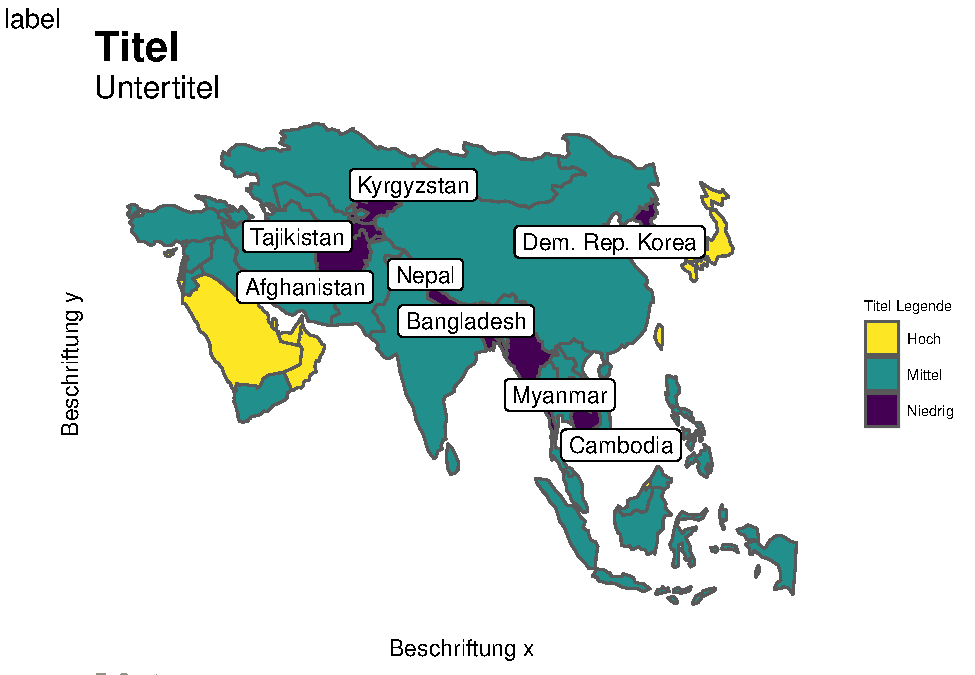
\includegraphics{ggplot2_files/figure-latex/unnamed-chunk-9-1.pdf}

Lorem ipsum dolor sit amet, consetetur sadipscing elitr, sed diam nonumy
eirmod tempor invidunt ut labore et dolore magna aliquyam erat, sed diam
voluptua. At vero eos et accusam et justo duo dolores et ea rebum.

\columnbreak

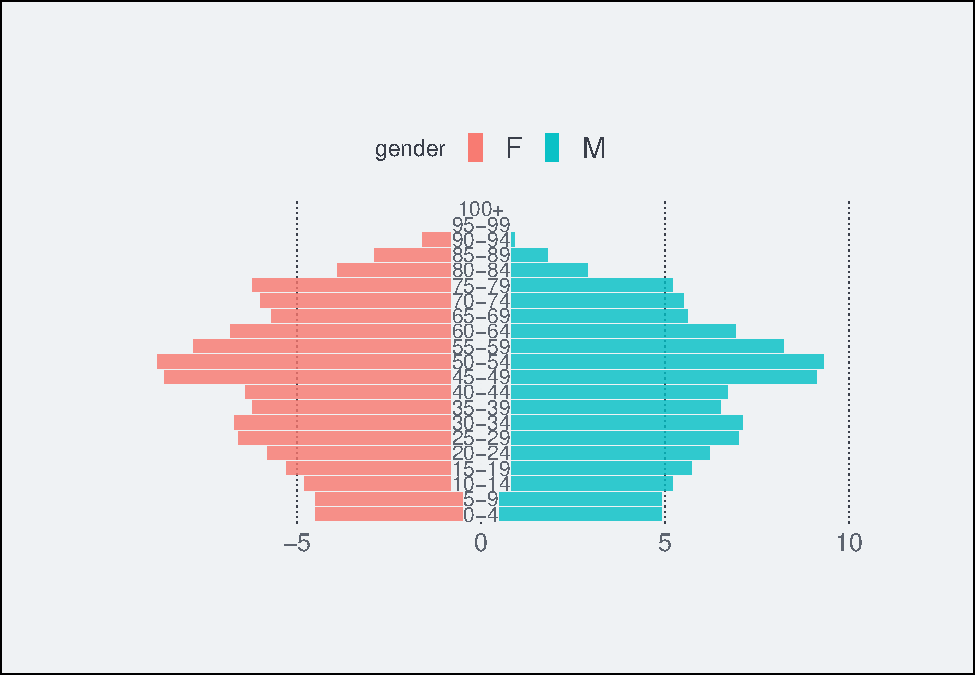
\includegraphics{ggplot2_files/figure-latex/unnamed-chunk-10-1.pdf}

Lorem ipsum dolor sit amet, consetetur sadipscing elitr, sed diam nonumy
eirmod tempor invidunt ut labore et dolore magna aliquyam erat, sed diam
voluptua. At vero eos et accusam et justo duo dolores et ea rebum.

\end {multicols}

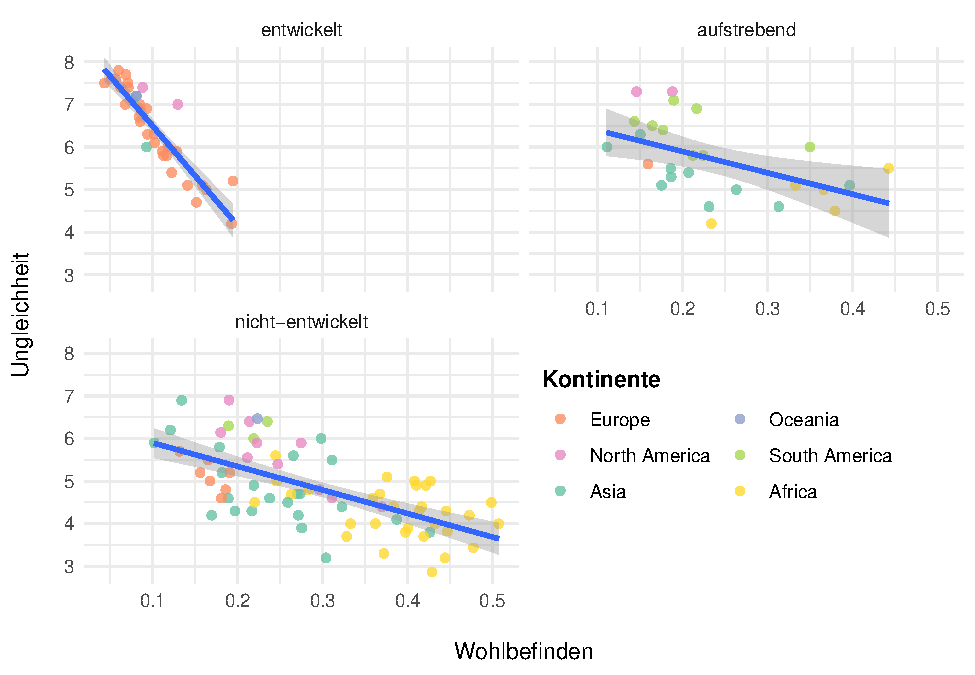
\includegraphics{ggplot2_files/figure-latex/unnamed-chunk-11-1.pdf}

\hypertarget{spaltiges-layout}{%
\subsection{1 Spaltiges Layout}\label{spaltiges-layout}}

\hypertarget{alternativen-zur-population-pyramid}{%
\paragraph{Alternativen zur Population
Pyramid}\label{alternativen-zur-population-pyramid}}

\begin{Shaded}
\begin{Highlighting}[]
\NormalTok{plotBarGrouped}
\end{Highlighting}
\end{Shaded}

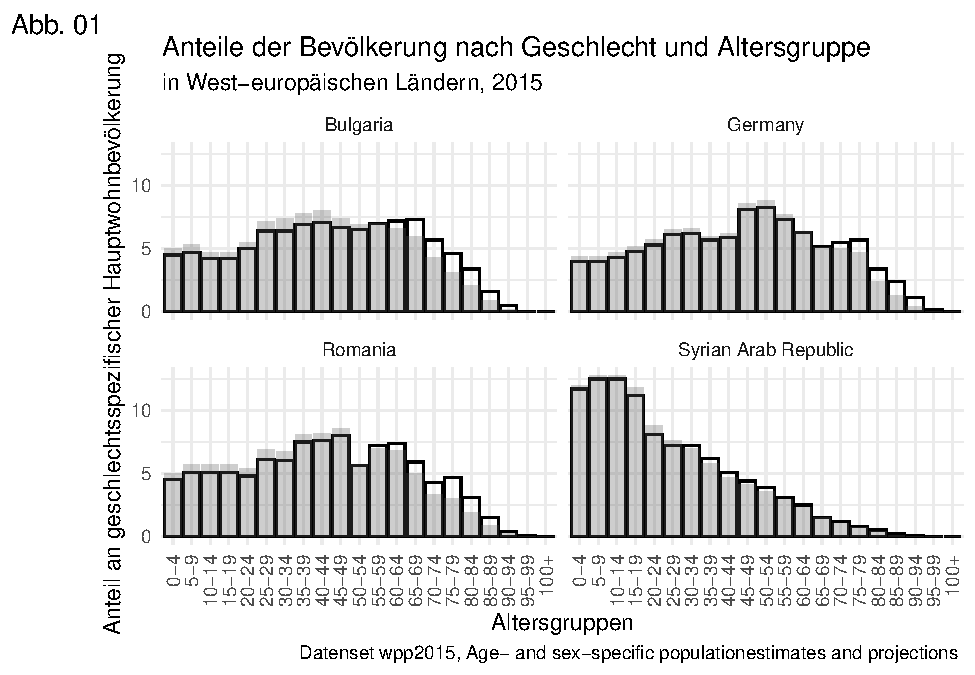
\includegraphics{ggplot2_files/figure-latex/unnamed-chunk-12-1.pdf}

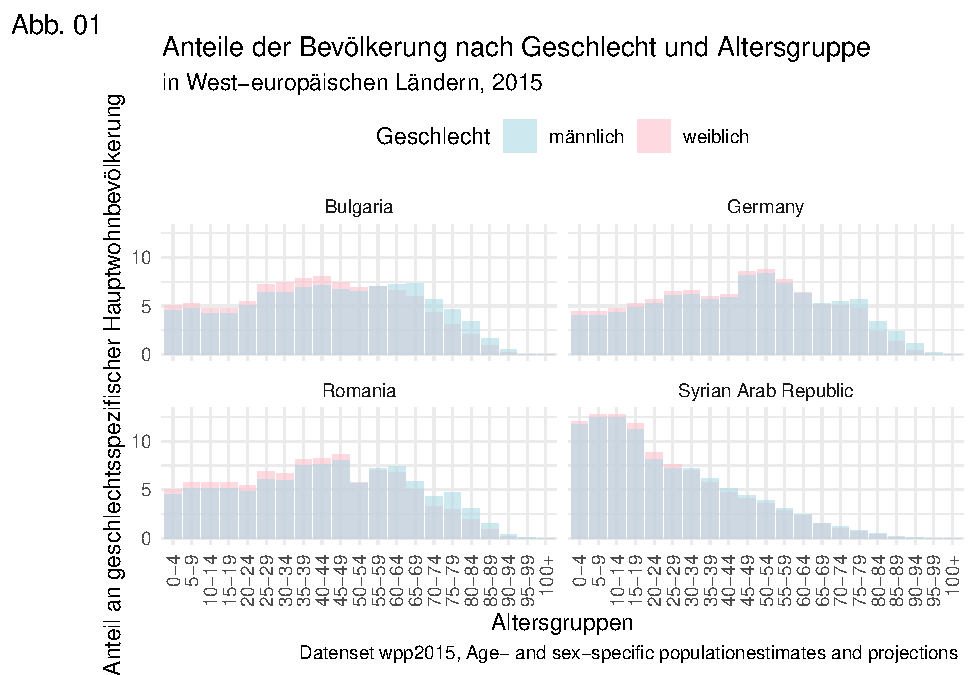
\includegraphics{ggplot2_files/figure-latex/unnamed-chunk-13-1.pdf}
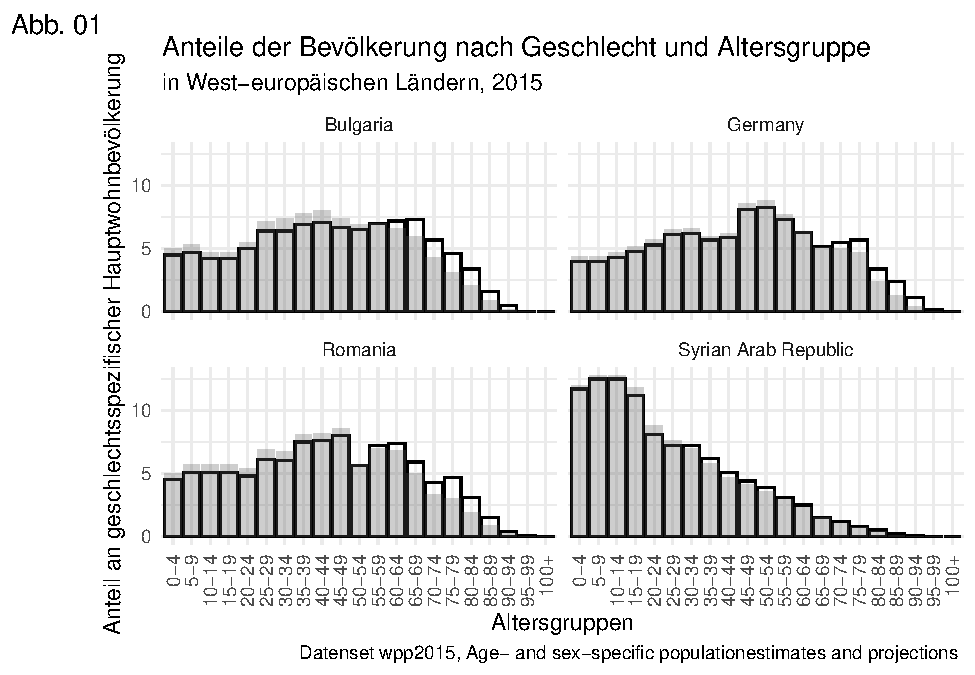
\includegraphics{ggplot2_files/figure-latex/unnamed-chunk-14-1.pdf}

\end{document}
